% Options for packages loaded elsewhere
\PassOptionsToPackage{unicode}{hyperref}
\PassOptionsToPackage{hyphens}{url}
%
\documentclass[
]{article}
\title{표의 시각화}
\author{}
\date{\vspace{-2.5em}}

\usepackage{amsmath,amssymb}
\usepackage{lmodern}
\usepackage{iftex}
\ifPDFTeX
  \usepackage[T1]{fontenc}
  \usepackage[utf8]{inputenc}
  \usepackage{textcomp} % provide euro and other symbols
\else % if luatex or xetex
  \usepackage{unicode-math}
  \defaultfontfeatures{Scale=MatchLowercase}
  \defaultfontfeatures[\rmfamily]{Ligatures=TeX,Scale=1}
\fi
% Use upquote if available, for straight quotes in verbatim environments
\IfFileExists{upquote.sty}{\usepackage{upquote}}{}
\IfFileExists{microtype.sty}{% use microtype if available
  \usepackage[]{microtype}
  \UseMicrotypeSet[protrusion]{basicmath} % disable protrusion for tt fonts
}{}
\makeatletter
\@ifundefined{KOMAClassName}{% if non-KOMA class
  \IfFileExists{parskip.sty}{%
    \usepackage{parskip}
  }{% else
    \setlength{\parindent}{0pt}
    \setlength{\parskip}{6pt plus 2pt minus 1pt}}
}{% if KOMA class
  \KOMAoptions{parskip=half}}
\makeatother
\usepackage{xcolor}
\IfFileExists{xurl.sty}{\usepackage{xurl}}{} % add URL line breaks if available
\IfFileExists{bookmark.sty}{\usepackage{bookmark}}{\usepackage{hyperref}}
\hypersetup{
  pdftitle={표의 시각화},
  hidelinks,
  pdfcreator={LaTeX via pandoc}}
\urlstyle{same} % disable monospaced font for URLs
\usepackage[margin=1in]{geometry}
\usepackage{color}
\usepackage{fancyvrb}
\newcommand{\VerbBar}{|}
\newcommand{\VERB}{\Verb[commandchars=\\\{\}]}
\DefineVerbatimEnvironment{Highlighting}{Verbatim}{commandchars=\\\{\}}
% Add ',fontsize=\small' for more characters per line
\usepackage{framed}
\definecolor{shadecolor}{RGB}{248,248,248}
\newenvironment{Shaded}{\begin{snugshade}}{\end{snugshade}}
\newcommand{\AlertTok}[1]{\textcolor[rgb]{0.94,0.16,0.16}{#1}}
\newcommand{\AnnotationTok}[1]{\textcolor[rgb]{0.56,0.35,0.01}{\textbf{\textit{#1}}}}
\newcommand{\AttributeTok}[1]{\textcolor[rgb]{0.77,0.63,0.00}{#1}}
\newcommand{\BaseNTok}[1]{\textcolor[rgb]{0.00,0.00,0.81}{#1}}
\newcommand{\BuiltInTok}[1]{#1}
\newcommand{\CharTok}[1]{\textcolor[rgb]{0.31,0.60,0.02}{#1}}
\newcommand{\CommentTok}[1]{\textcolor[rgb]{0.56,0.35,0.01}{\textit{#1}}}
\newcommand{\CommentVarTok}[1]{\textcolor[rgb]{0.56,0.35,0.01}{\textbf{\textit{#1}}}}
\newcommand{\ConstantTok}[1]{\textcolor[rgb]{0.00,0.00,0.00}{#1}}
\newcommand{\ControlFlowTok}[1]{\textcolor[rgb]{0.13,0.29,0.53}{\textbf{#1}}}
\newcommand{\DataTypeTok}[1]{\textcolor[rgb]{0.13,0.29,0.53}{#1}}
\newcommand{\DecValTok}[1]{\textcolor[rgb]{0.00,0.00,0.81}{#1}}
\newcommand{\DocumentationTok}[1]{\textcolor[rgb]{0.56,0.35,0.01}{\textbf{\textit{#1}}}}
\newcommand{\ErrorTok}[1]{\textcolor[rgb]{0.64,0.00,0.00}{\textbf{#1}}}
\newcommand{\ExtensionTok}[1]{#1}
\newcommand{\FloatTok}[1]{\textcolor[rgb]{0.00,0.00,0.81}{#1}}
\newcommand{\FunctionTok}[1]{\textcolor[rgb]{0.00,0.00,0.00}{#1}}
\newcommand{\ImportTok}[1]{#1}
\newcommand{\InformationTok}[1]{\textcolor[rgb]{0.56,0.35,0.01}{\textbf{\textit{#1}}}}
\newcommand{\KeywordTok}[1]{\textcolor[rgb]{0.13,0.29,0.53}{\textbf{#1}}}
\newcommand{\NormalTok}[1]{#1}
\newcommand{\OperatorTok}[1]{\textcolor[rgb]{0.81,0.36,0.00}{\textbf{#1}}}
\newcommand{\OtherTok}[1]{\textcolor[rgb]{0.56,0.35,0.01}{#1}}
\newcommand{\PreprocessorTok}[1]{\textcolor[rgb]{0.56,0.35,0.01}{\textit{#1}}}
\newcommand{\RegionMarkerTok}[1]{#1}
\newcommand{\SpecialCharTok}[1]{\textcolor[rgb]{0.00,0.00,0.00}{#1}}
\newcommand{\SpecialStringTok}[1]{\textcolor[rgb]{0.31,0.60,0.02}{#1}}
\newcommand{\StringTok}[1]{\textcolor[rgb]{0.31,0.60,0.02}{#1}}
\newcommand{\VariableTok}[1]{\textcolor[rgb]{0.00,0.00,0.00}{#1}}
\newcommand{\VerbatimStringTok}[1]{\textcolor[rgb]{0.31,0.60,0.02}{#1}}
\newcommand{\WarningTok}[1]{\textcolor[rgb]{0.56,0.35,0.01}{\textbf{\textit{#1}}}}
\usepackage{graphicx}
\makeatletter
\def\maxwidth{\ifdim\Gin@nat@width>\linewidth\linewidth\else\Gin@nat@width\fi}
\def\maxheight{\ifdim\Gin@nat@height>\textheight\textheight\else\Gin@nat@height\fi}
\makeatother
% Scale images if necessary, so that they will not overflow the page
% margins by default, and it is still possible to overwrite the defaults
% using explicit options in \includegraphics[width, height, ...]{}
\setkeys{Gin}{width=\maxwidth,height=\maxheight,keepaspectratio}
% Set default figure placement to htbp
\makeatletter
\def\fps@figure{htbp}
\makeatother
\setlength{\emergencystretch}{3em} % prevent overfull lines
\providecommand{\tightlist}{%
  \setlength{\itemsep}{0pt}\setlength{\parskip}{0pt}}
\setcounter{secnumdepth}{-\maxdimen} % remove section numbering
\usepackage{amsmath}
\usepackage{booktabs}
\usepackage{caption}
\usepackage{longtable}
\ifLuaTeX
  \usepackage{selnolig}  % disable illegal ligatures
\fi

\begin{document}
\maketitle

데이터 시각화를 한다고 하면 대부분 떠올리는 작업이 그래프를 그리는
작업이다. 그래서 데이터 시각화를 시작할 때는 먼저 데이터를 대상으로
할지, 어떤 그래프를 써서 데이터를 예쁘고 직관적으로 표현할지를 고민하게
된다. 하지만 데이터 시각화 결과가 들어갈 보고문서에는 대부분 그래프와
함께 표가 들어가는 경우가 대부분이지만 데이터를 설명하는 데이터 시각화를
해야할 때 많은 사람들은 표까지 생각하지는 않는 듯하다. 인터넷 상의 표의
정의\footnote{\url{https://ko.wikipedia.org/wiki/\%ED\%91\%9C}}를 보면
'시각적 의사소통과 자료의 정렬 양식'으로 나와 있다. 결국 표도 데이터
시각화의 일부인 것이다.

표는 데이터를 직접적으로 표현한다는 점에서 그래프나 플롯과는 다르다.
데이터를 직접 표현하기 때문에 데이터를 정확하게 표현하지만 데이터의
전체적인 흐름이나 분포를 알아보기에는 적절치 않다. 하지만 그래프나
플롯은 정확한 데이터를 알아보기 힘들다는 점에서 표와 그래프, 플롯은 상호
보완적으로 사용되어야 한다.

\hypertarget{uxd45ctableuxb780}{%
\section{표(table)란?}\label{uxd45ctableuxb780}}

표는 행과 열로 이루어진 데이터의 모음이다. 행은 각각의 개별 사례2나 개별
사례를 적절히 그루핑한 요약된 데이터가 표현된다. 열은 각각의 사례를
설명하기 위해 필요한 속성이 나열된다. 행과 열은 이 만나는 곳이 사용자가
알고 싶어하는 데이터가 위치하고 이 곳을 칸, 혹은 셀이라고 한다.

표는 그 구성 방법에 따라 1차원 표와 다차원 표로 구성된다. 1차원 표는
단순히 데이터의 나열인 경우를 말한다. 이런 테이블을 '단순 표(simple
table)'이라고도 한다. 다차원 표는 1차원 표를 적절한 변환(추상화)하여
표에서 제공하는 몇가지 차원의 정보를 모두 가져야 데이터를 해석할 수 있는
표를 말한다. 다차원 표 중에서 가장 흔하게 보이는 표가 2차원 표,
교차표(cross table)이다. 2차원 표는 행(X축)과 열(Y축)의 정보를 가지고
해당 칸(셀)의 정보를 해석할 수 있다.

아래의 그림은 1차원 표와 2차원 표의 예를 보이고 있다.

\begin{figure}
\centering
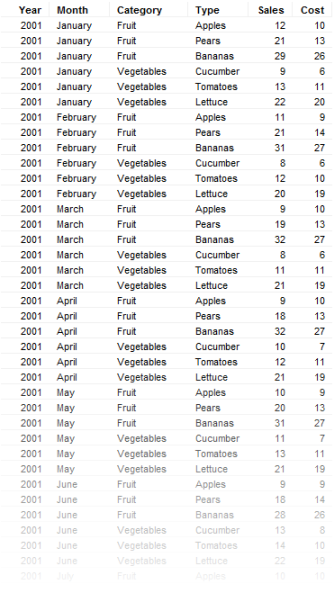
\includegraphics{cross_example_table.png}
\caption{\url{https://docs.tibco.com/pub/spotfire/6.5.2/doc/html/images/cross_example_table.png}}
\end{figure}

\begin{figure}
\centering
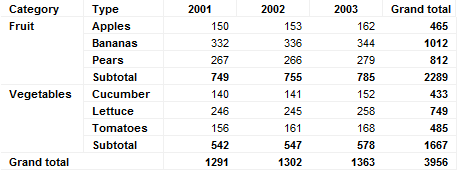
\includegraphics{cross_example_cross_table.png}
\caption{\url{https://docs.tibco.com/pub/spotfire/6.5.2/doc/html/images/cross_example_cross_table.png}}
\end{figure}

위의 그림에서 보면 1차원 표의 경우는 데이터를 설명하는 속성이 위쪽에만
설정되어 있다. 하지만 2차원 표의 경우는 데이터를 설명하는 속성이 위쪽과
왼쪽에 모두 설정되어 있다. 특정 칸의 데이터를 해석하기 위해서는 행과
열의 속성 정보를 모두 알아야 한다는 것이다.

1차원 표의 장점은 데이터를 원본 차원에서 확인 할 수 있다는 점이다. 반면
데이터의 행이 길어질 수 있어 보고서에 수록하는 것인 적절치 않을 때가
있다. 하지만 다차원 표의 가장 큰 장점은 데이터를 요약하고 구조화하였기
때문에 대량의 데이터의 특성을 간략히 표현했다는 점이다. 하지만 데이터를
요약하는 방식에 따라 전달되는 정보가 제한적일 수 있다는 단점이 있다.

표의 구성 방법과 요소는 사용자가 표현하고 싶은 데이터와 형태에 따라
표현방식이 매우 다르기 때문에 어느 하나로 정의하기가 어렵다. 다음 그림은
논문의 작성에서 대표적으로 사용되는 미국 심리학회의 표 구성
가이드라인이다.

\begin{figure}
\centering
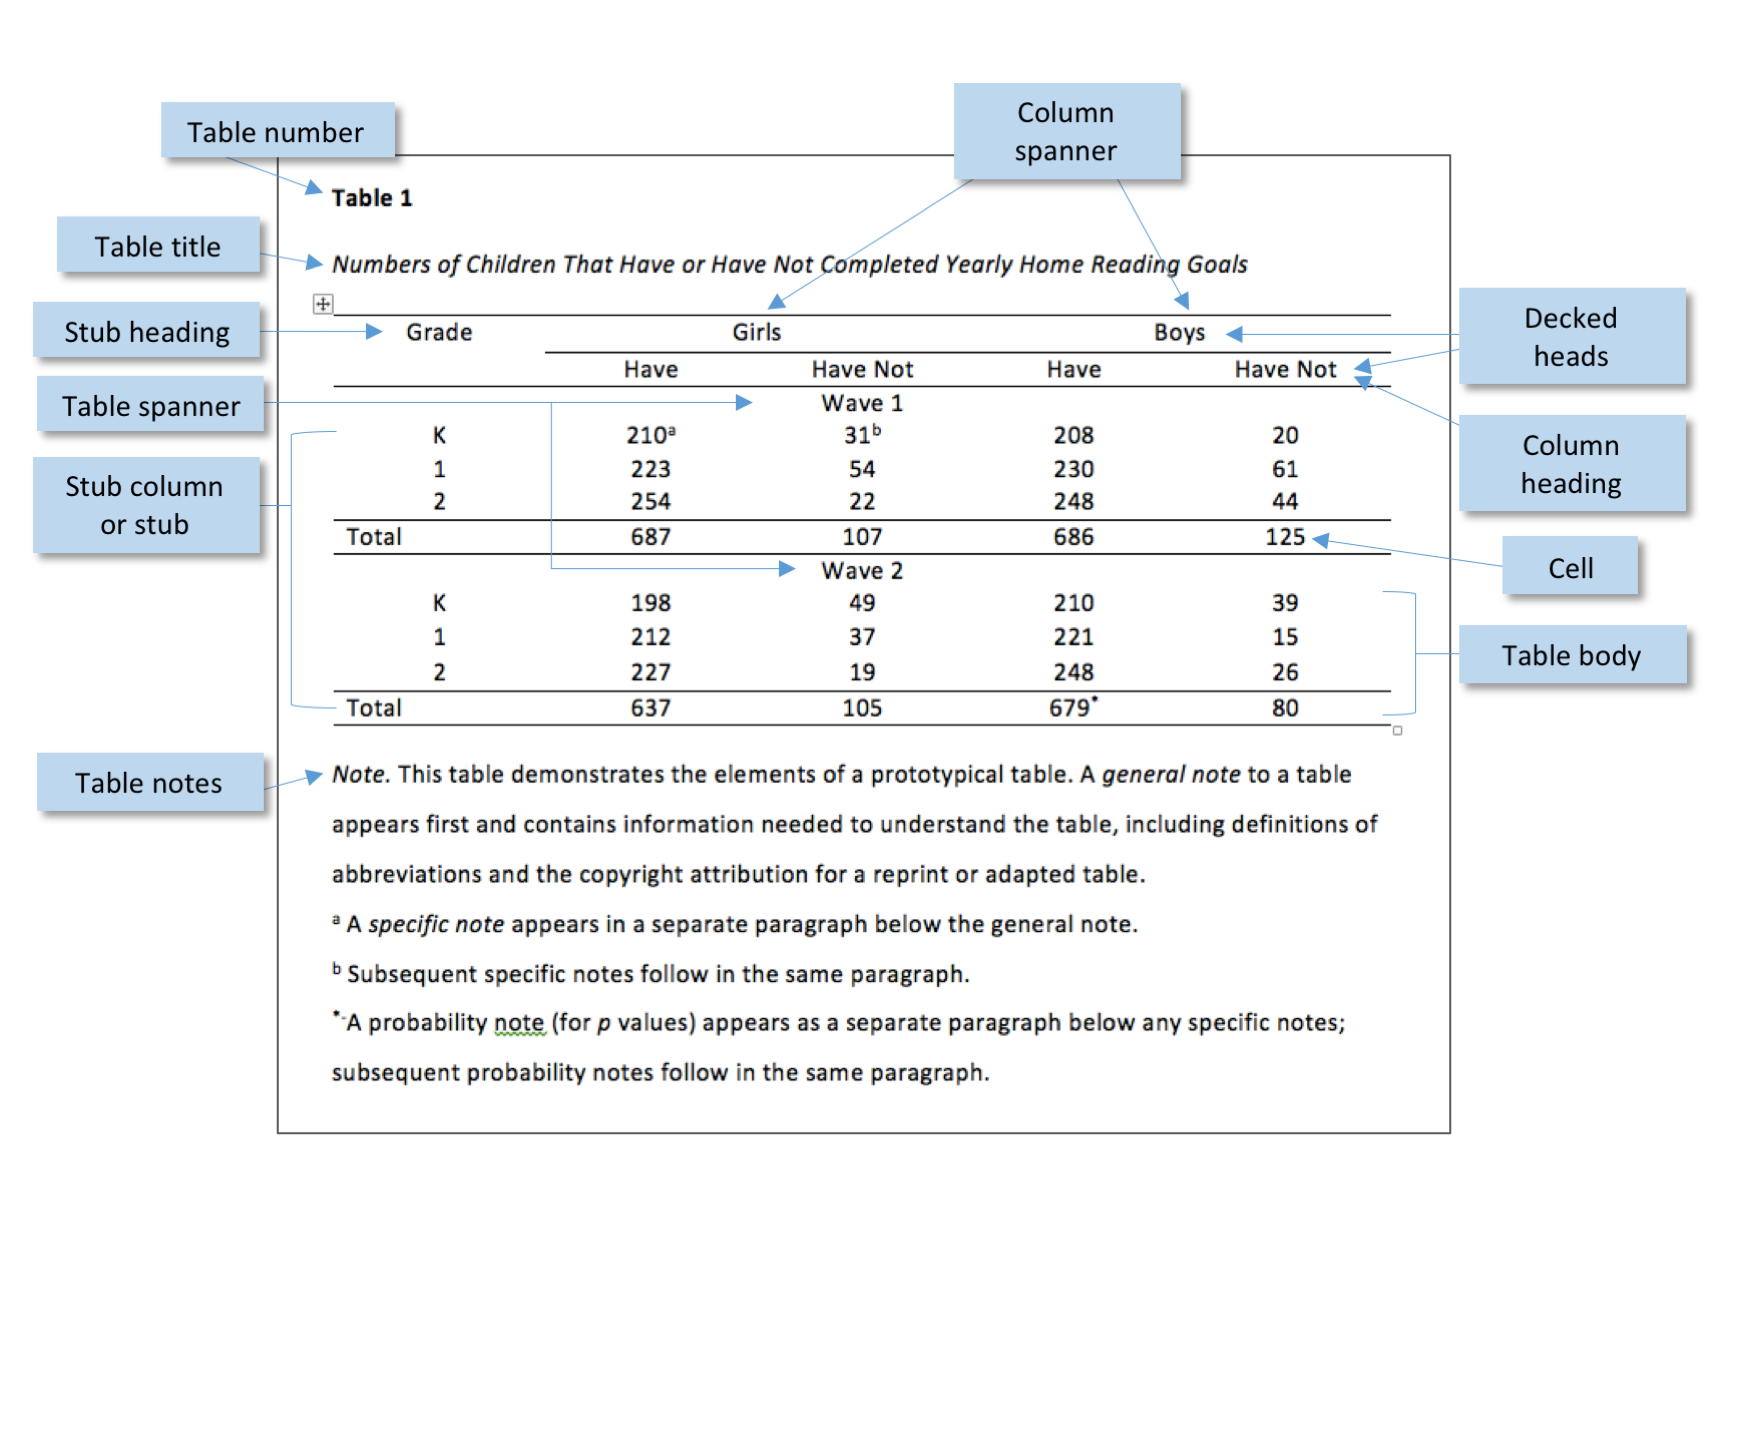
\includegraphics{apa.png}
\caption{\url{https://libapps.s3.amazonaws.com/customers/836/qu/e1d262992c7ea1e2aa109305faf24d59.png}}
\end{figure}

모든 표를 APA 가이드라인에 맞춰 그릴 수는 없겠지만 APA 가이드라인을 보면
표에 꼭 들어가야 할 몇가지 요소들을 알 수 있다.

\begin{itemize}
\item
  제목(Title) : 표에서 표현하고 있는 데이터를 대표하는 제목
\item
  헤드(Heading) : 표에서 제시하고 있는 사례들의 속성값들에 대한 이름이
  표현된 표 가로축의 맨 위줄
\item
  스텁(Stub) : 표에서 사례를 표현하는 세로축의 묶음
\item
  스패너(Spanner) : 표의 특성을 표현하는 가로축 중에 유사한 특성의 묶음
\item
  몸체(Body) : 표의 헤드와 스텁으로 감싸고 있는 데이터가 표현된 셀들이
  표현된 부분
\end{itemize}

실무에서 표를 그릴 때 가장 많이 사용하는 툴은 아마도 MS-Excel일 것이다.
SpreadSheet로 거의 유일하게(?) 살아남은 이 툴은 표를 그리는 WYSYWYG(What
You See IS Wat You Get) 툴로 거의 모든 Spreadsheet를 없애버렸다고 해도
과언이 아닐 듯 하다. 어쨌던 엑셀은 표를 그리는데 매우 특화된 툴임에는
틀림없고 초보자들도 쉽게 사용할 수 있지만 사용하다보면 몇가지 단점을
만날 수 있다.

가장 큰 단점이 반복된 작업을 하기가 어렵다는 점이다. 이는 WYSIWIG 툴들이
가지는 공통된 단점이다. 표를 쉽게 만들 수 있지만 유사한 표를 다시
만들어야 하는 경우 반복된 작업을 수행해야하고 반복된 작업을 꼼꼼히
기록해두지 않으면 동일한 표를 만들기 어렵다. 또 하나의 단점이 기초
데이터의 구조가 업데이트 되면 표를 다시 그려야 하는 경우가 발생한다는
점이다. 기초 데이터의 열 이름이 바뀌거나 열이 추가, 삭제되면 이
데이터로부터 파생된 표가 정상적으로 표현되지 않는다는 것이다. 이러한
문제는 엑셀을 사용해 본 사용자라면 한번쯤, 아니 자주 겪는 문제일 것이다.

이제 엑셀에서 탈피해서 R에서 표를 그려보자. R에서도 아주 훌륭한, 그리고
예쁘게 표를 그릴 수 있는 다양한 방법을 제공한다. R로 표를 그려보면
반복된 작업을 할 필요가 없다는 점에서, 기초 데이터의 업데이트가 발생해도
바로 반영할 수 있다는 점, 표를 세세하게 다룰 수 있다는 점에서 엑셀로
다시 돌아갈 수 없을 수도 있다.

\hypertarget{gt-uxd328uxd0a4uxc9c0}{%
\section{\texorpdfstring{\texttt{gt}
패키지}{gt 패키지}}\label{gt-uxd328uxd0a4uxc9c0}}

R에서 표를 만들기 위해 사용되는 패키지 중에 하나가 \texttt{gt}
패키지이다. \texttt{gt} 패키지는 표의 세부 구성들을 상세히 구분하고
이들을 구조적으로 조화롭게 구성시켜서 표를 만드는 다양한 함수와 매개
변수들을 제공한다. \texttt{gt} 패키지에서 사용하는 표의 세부 파트는
다음의 그림과 같다.

\begin{figure}
\centering
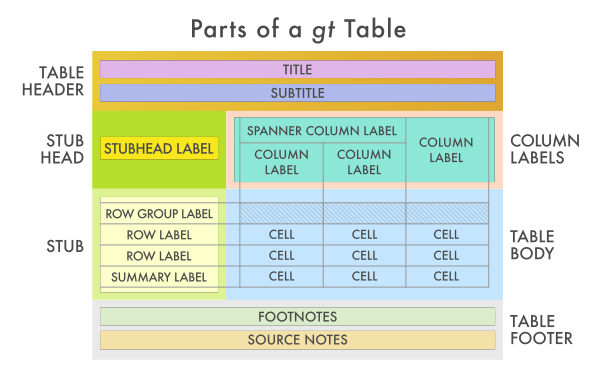
\includegraphics{gt_parts_of_a_table.svg}
\caption{\href{https://gt.rstudio.com/reference/figures/gt_parts_of_a_table.svg}{https://gt.rstudio.com/reference/figures/gt\_parts\_of\_a\textbackslash\textbackslash\textbackslash\_table.svg}}
\end{figure}

표의 구성을 보면 앞에서 살펴보았던 APA 가이드라인상의 표와 유사한 형태를
보인다. 이와 같이 표를 세부적인 파트로 구분하고 이들을 각각 설정함으로써
표를 만들 수 있다.

\texttt{gt} 패키지에서 권장하는 표 생성 방식은 다음의 그림과 같다

\begin{figure}
\centering
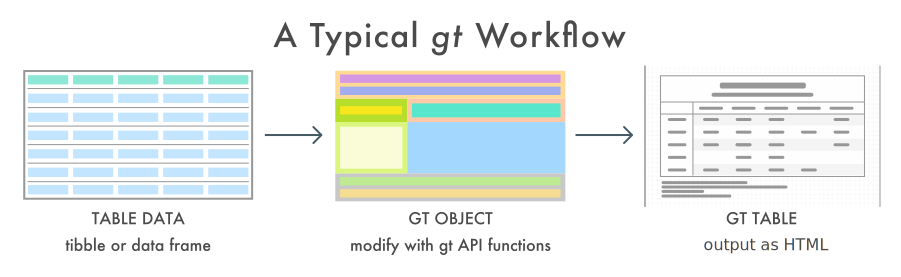
\includegraphics{gt_workflow_diagram.svg}
\caption{\url{https://gt.rstudio.com/reference/figures/gt_workflow_diagram.svg}}
\end{figure}

우선 표를 만들기 위한 기초 데이터를 생성해야 한다. \texttt{gt} 패키지로
생성되는 표는 \texttt{tidyverse} 방식을 준용하여 생성하는 것이 편하다.
따라서 \texttt{gt} 표를 생성하기 위해 만드는 기초 데이터도
\texttt{tidyverse} 의 \texttt{tibble} 이나 R의 기초 데이터 셋인
\texttt{data.frame} 으로 생성한다. 이렇게 생성된 기초 데이터 셋은
\texttt{gt} 객체로 변환되고 \texttt{gt} 패키지에서 제공되는 다양한
함수와 매개변수를 설정하여 사용자가 원하는 형태의 표로 만들게 된다.
마지막으로 이 표를 다른 문서에서 활용하기 위해 html, pdf 등의 문서로
변환하여 활용한다.

우선 \texttt{gt} 패키지를 사용하기 위해서는 \texttt{gt} 패키지를
설치하고 로딩하여야 한다.

\begin{Shaded}
\begin{Highlighting}[]
\ControlFlowTok{if}\NormalTok{(}\SpecialCharTok{!}\FunctionTok{require}\NormalTok{(}\StringTok{\textquotesingle{}gt\textquotesingle{}}\NormalTok{)) \{}
  \FunctionTok{install.packages}\NormalTok{(}\StringTok{\textquotesingle{}gt\textquotesingle{}}\NormalTok{)}
  \FunctionTok{library}\NormalTok{(gt)}
\NormalTok{\}}
\end{Highlighting}
\end{Shaded}

이번 장에서 사용할 데이터는 앞 장에서 생성한 df\_취업통계 데이터를
사용하겠다. 최종 생성될 표는 각각의 과정구분에 따라 편성된 대계열
학과들에 대한 취업 정보를 요약한 표이다. 표에서는 각각의 열을 과정구분로
구분(Stub)하고, 특성으로 표현되는 열은 졸업자, 취업자, 취업률 등 졸업 후
상황별 학생수를 표기하는데 취업 상세 학생과 비취업 상세 학생으로 열을
묶어(Spanner)하고 소계와 총계가 나타나는 표를 그리겠다.

\hypertarget{uxb370uxc774uxd130-uxc804uxcc98uxb9ac}{%
\subsection{데이터 전처리}\label{uxb370uxc774uxd130-uxc804uxcc98uxb9ac}}

우선 목표한 표를 만들기 위해 가진 데이터를 전처리하는 과정이 필요하다.
우선 추가적으로 필요한 열을 생성한다. 개별 학과별로 저장된 원본 데이터를
대계열별, 과정구분별로 요약(Summarise)하고 표현될 순서를 설정하기 위해
팩터로 레벨을 설정하도록 하겠다.

\begin{Shaded}
\begin{Highlighting}[]
\DocumentationTok{\#\# df\_취업통계를 전처리하여 df\_gt로 저장}
\NormalTok{df\_gt }\OtherTok{\textless{}{-}}\NormalTok{ df\_취업통계 }\SpecialCharTok{|}\ErrorTok{\textgreater{}}
  \DocumentationTok{\#\# 과정구분과 대계열로 그루핑}
  \FunctionTok{group\_by}\NormalTok{(과정구분, 대계열) }\SpecialCharTok{|}\ErrorTok{\textgreater{}}
  \DocumentationTok{\#\# 각각의 열단위로 합계값으로 요약된 열 생성 }
  \FunctionTok{summarise}\NormalTok{(졸업자 }\OtherTok{=} \FunctionTok{sum}\NormalTok{(졸업자\_계), }
\NormalTok{            취업자 }\OtherTok{=} \FunctionTok{sum}\NormalTok{(취업자\_합계\_계), }
\NormalTok{            교외취업자 }\OtherTok{=} \FunctionTok{sum}\NormalTok{(취업자\_교외취업자\_계), }
\NormalTok{            교내취업자 }\OtherTok{=} \FunctionTok{sum}\NormalTok{(취업자\_교내취업자\_계), }
\NormalTok{            해외취업자 }\OtherTok{=} \FunctionTok{sum}\NormalTok{(취업자\_해외취업자\_계), }
\NormalTok{            농림어업종사자 }\OtherTok{=} \FunctionTok{sum}\NormalTok{(취업자\_농림어업종사자\_계), }
\NormalTok{            개인창작활동종사자 }\OtherTok{=} \FunctionTok{sum}\NormalTok{(취업자\_개인창작활동종사자\_계), }
\NormalTok{            일인창사업자 }\OtherTok{=} \FunctionTok{sum}\NormalTok{(}\StringTok{\textasciigrave{}}\AttributeTok{취업자\_1인창(사)업자\_계}\StringTok{\textasciigrave{}}\NormalTok{), }
\NormalTok{            프리랜서 }\OtherTok{=} \FunctionTok{sum}\NormalTok{(취업자\_프리랜서\_계), }
\NormalTok{            진학자 }\OtherTok{=} \FunctionTok{sum}\NormalTok{(진학자\_계), }
\NormalTok{            입대자 }\OtherTok{=} \FunctionTok{sum}\NormalTok{(입대자),}
\NormalTok{            취업불가능자 }\OtherTok{=} \FunctionTok{sum}\NormalTok{(취업불가능자\_계), }
\NormalTok{            외국인유학생 }\OtherTok{=} \FunctionTok{sum}\NormalTok{(외국인유학생\_계), }
\NormalTok{            제외인정자 }\OtherTok{=} \FunctionTok{sum}\NormalTok{(제외인정자\_계), }
\NormalTok{            기타 }\OtherTok{=} \FunctionTok{sum}\NormalTok{(기타\_계), }
\NormalTok{            미상 }\OtherTok{=} \FunctionTok{sum}\NormalTok{(미상\_계), }
    \DocumentationTok{\#\# 백분률인 취업률은 그 자체로 합계나 평균을 낼 수 없으니 각 그룹별로 재계산}
\NormalTok{            취업률 }\OtherTok{=}\NormalTok{ 취업자 }\SpecialCharTok{/}\NormalTok{ (졸업자 }\SpecialCharTok{{-}}\NormalTok{ (진학자}\SpecialCharTok{+}\NormalTok{입대자}\SpecialCharTok{+}\NormalTok{취업불가능자}\SpecialCharTok{+}\NormalTok{외국인유학생}\SpecialCharTok{+}\NormalTok{제외인정자))) }\SpecialCharTok{|}\ErrorTok{\textgreater{}}
  \DocumentationTok{\#\# 최종결과는 그룹 설정을 제거}
  \FunctionTok{ungroup}\NormalTok{()  }\SpecialCharTok{|}\ErrorTok{\textgreater{}} 
  \FunctionTok{arrange}\NormalTok{(과정구분)}

\FunctionTok{head}\NormalTok{(df\_gt, }\DecValTok{10}\NormalTok{)}
\end{Highlighting}
\end{Shaded}

\begin{verbatim}
## # A tibble: 10 x 19
##    과정구분 대계열 졸업자 취업자 교외취업자 교내취업자 해외취업자 농림어업종사자
##    <chr>    <chr>   <dbl>  <dbl>      <dbl>      <dbl>      <dbl>          <dbl>
##  1 대학과정 공학~   83953  47789      44414       1016        179              5
##  2 대학과정 교육~   19733   9258       8156        239          6              1
##  3 대학과정 사회~   90304  47721      42979       1198        242             23
##  4 대학과정 예체~   36247  19104      13607        619         68              3
##  5 대학과정 의약~   25386  20014      19570        126          7              0
##  6 대학과정 인문~   37864  16681      13722        772        210              5
##  7 대학과정 자연~   37555  17648      15454        616         36             46
##  8 대학원~  공학~   13978   9348       8766        396         35              0
##  9 대학원~  교육~    2694   1763       1550         69          0              1
## 10 대학원~  사회~    8178   4141       3724         90          2              3
## # ... with 11 more variables: 개인창작활동종사자 <dbl>, 일인창사업자 <dbl>,
## #   프리랜서 <dbl>, 진학자 <dbl>, 입대자 <dbl>, 취업불가능자 <dbl>,
## #   외국인유학생 <dbl>, 제외인정자 <dbl>, 기타 <dbl>, 미상 <dbl>, 취업률 <dbl>
\end{verbatim}

\begin{Shaded}
\begin{Highlighting}[]
\DocumentationTok{\#\# 과정구분의 순서를 맞추기 위해 과정구분을 팩터로 설정하고 레벨의 순서를 설정}
\NormalTok{df\_gt}\SpecialCharTok{$}\NormalTok{과정구분 }\OtherTok{\textless{}{-}} \FunctionTok{fct\_relevel}\NormalTok{(df\_gt}\SpecialCharTok{$}\NormalTok{과정구분, }\StringTok{\textquotesingle{}전문대학과정\textquotesingle{}}\NormalTok{, }\StringTok{\textquotesingle{}대학과정\textquotesingle{}}\NormalTok{, }\StringTok{\textquotesingle{}대학원과정\textquotesingle{}}\NormalTok{)}

\DocumentationTok{\#\# 대계열의 순서를 맞추기 위해 과정구분을 팩터로 설정하고 레벨의 순서를 설정}
\NormalTok{df\_gt}\SpecialCharTok{$}\NormalTok{대계열 }\OtherTok{\textless{}{-}} \FunctionTok{fct\_relevel}\NormalTok{(df\_gt}\SpecialCharTok{$}\NormalTok{대계열, }\StringTok{\textquotesingle{}인문계열\textquotesingle{}}\NormalTok{, }\StringTok{\textquotesingle{}사회계열\textquotesingle{}}\NormalTok{, }\StringTok{\textquotesingle{}교육계열\textquotesingle{}}\NormalTok{, }\StringTok{\textquotesingle{}자연계열\textquotesingle{}}\NormalTok{, }\StringTok{\textquotesingle{}공학계열\textquotesingle{}}\NormalTok{, }\StringTok{\textquotesingle{}의약계열\textquotesingle{}}\NormalTok{, }\StringTok{\textquotesingle{}예체능계열\textquotesingle{}}\NormalTok{)}

\DocumentationTok{\#\# 백분률인 취업률은 그 자체로 합계나 평균을 낼 수 없으니 각 소계 그룹별로 재계산하여 dt\_gt\_summary에 저장}
\NormalTok{df\_gt\_summary }\OtherTok{\textless{}{-}}\NormalTok{ df\_gt }\SpecialCharTok{|}\ErrorTok{\textgreater{}} \FunctionTok{group\_by}\NormalTok{(대계열) }\SpecialCharTok{|}\ErrorTok{\textgreater{}} 
  \FunctionTok{summarise}\NormalTok{(취업률 }\OtherTok{=} \FunctionTok{sum}\NormalTok{(취업자) }\SpecialCharTok{/}\NormalTok{ (}\FunctionTok{sum}\NormalTok{(졸업자) }\SpecialCharTok{{-}}\NormalTok{ (}\FunctionTok{sum}\NormalTok{(진학자)}\SpecialCharTok{+}\FunctionTok{sum}\NormalTok{(입대자)}\SpecialCharTok{+}\FunctionTok{sum}\NormalTok{(취업불가능자)}\SpecialCharTok{+}\FunctionTok{sum}\NormalTok{(외국인유학생)}\SpecialCharTok{+}\FunctionTok{sum}\NormalTok{(제외인정자))))}

\DocumentationTok{\#\# 백분률인 취업률은 그 자체로 합계나 평균을 낼 수 없으니 각 총계로 재계산하여 dt\_gt\_grand\_summary에 저장}
\NormalTok{df\_gt\_grand\_summary }\OtherTok{\textless{}{-}}\NormalTok{ df\_gt }\SpecialCharTok{|}\ErrorTok{\textgreater{}}  
  \FunctionTok{summarise}\NormalTok{(취업률 }\OtherTok{=} \FunctionTok{sum}\NormalTok{(취업자) }\SpecialCharTok{/}\NormalTok{ (}\FunctionTok{sum}\NormalTok{(졸업자) }\SpecialCharTok{{-}}\NormalTok{ (}\FunctionTok{sum}\NormalTok{(진학자)}\SpecialCharTok{+}\FunctionTok{sum}\NormalTok{(입대자)}\SpecialCharTok{+}\FunctionTok{sum}\NormalTok{(취업불가능자)}\SpecialCharTok{+}\FunctionTok{sum}\NormalTok{(외국인유학생)}\SpecialCharTok{+}\FunctionTok{sum}\NormalTok{(제외인정자))))}
\end{Highlighting}
\end{Shaded}

\hypertarget{gt-uxac1duxccb4-uxc0dduxc131uxd558uxae30}{%
\subsection{gt 객체
생성하기}\label{gt-uxac1duxccb4-uxc0dduxc131uxd558uxae30}}

gt 패키지를 사용하여 표를 그리려면 먼저 gt 패키지의 gt() 함수를 사용하여
gt 객체를 생성한다.(아래의 실행결과는 표의 일부만 표현하였다)

\begin{Shaded}
\begin{Highlighting}[]
\NormalTok{gt\_table1 }\OtherTok{\textless{}{-}}\NormalTok{ df\_gt }\SpecialCharTok{|}\ErrorTok{\textgreater{}}
  \FunctionTok{gt}\NormalTok{(}\AttributeTok{rowname\_col =} \StringTok{\textquotesingle{}과정구분\textquotesingle{}}\NormalTok{, }
     \AttributeTok{groupname\_col =} \StringTok{\textquotesingle{}대계열\textquotesingle{}}\NormalTok{)}

\NormalTok{gt\_table1}
\end{Highlighting}
\end{Shaded}

\captionsetup[table]{labelformat=empty,skip=1pt}
\begin{longtable}{lrrrrrrrrrrrrrrrrr}
\toprule
 & 졸업자 & 취업자 & 교외취업자 & 교내취업자 & 해외취업자 & 농림어업종사자 & 개인창작활동종사자 & 일인창사업자 & 프리랜서 & 진학자 & 입대자 & 취업불가능자 & 외국인유학생 & 제외인정자 & 기타 & 미상 & 취업률 \\ 
\midrule
\multicolumn{1}{l}{공학계열} \\ 
\midrule
대학과정 & 83953 & 47789 & 44414 & 1016 & 179 & 5 & 3 & 485 & 1687 & 7563 & 513 & 18 & 1235 & 328 & 25349 & 1158 & 0.6432244 \\ 
대학원과정 & 13978 & 9348 & 8766 & 396 & 35 & 0 & 0 & 44 & 107 & 1190 & 42 & 5 & 1807 & 7 & 1448 & 131 & 0.8554956 \\ 
전문대학과정 & 51049 & 30825 & 28325 & 391 & 139 & 57 & 250 & 328 & 1335 & 2649 & 2698 & 16 & 553 & 364 & 13591 & 353 & 0.6885345 \\ 
\midrule
\multicolumn{1}{l}{교육계열} \\ 
\midrule
대학과정 & 19733 & 9258 & 8156 & 239 & 6 & 1 & 50 & 65 & 741 & 604 & 318 & 2 & 92 & 396 & 8850 & 213 & 0.5053218 \\ 
대학원과정 & 2694 & 1763 & 1550 & 69 & 0 & 1 & 0 & 40 & 103 & 85 & 4 & 1 & 382 & 29 & 421 & 9 & 0.8039216 \\ 
전문대학과정 & 9660 & 7204 & 6893 & 95 & 0 & 9 & 35 & 37 & 135 & 662 & 52 & 1 & 23 & 110 & 1574 & 34 & 0.8175216 \\ 
\midrule
\multicolumn{1}{l}{사회계열} \\ 
\midrule
대학과정 & 90304 & 47721 & 42979 & 1198 & 242 & 23 & 6 & 835 & 2438 & 2209 & 397 & 25 & 5890 & 748 & 31911 & 1403 & 0.5888937 \\ 
대학원과정 & 8178 & 4141 & 3724 & 90 & 2 & 3 & 0 & 160 & 162 & 266 & 17 & 5 & 2717 & 7 & 893 & 132 & 0.8015873 \\ 
전문대학과정 & 39842 & 21248 & 18379 & 522 & 43 & 166 & 63 & 601 & 1474 & 3181 & 1390 & 18 & 581 & 730 & 12355 & 339 & 0.6260091 \\ 
\midrule
\multicolumn{1}{l}{예체능계열} \\ 
\midrule
대학과정 & 36247 & 19104 & 13607 & 619 & 68 & 3 & 686 & 838 & 3283 & 2099 & 764 & 9 & 1369 & 335 & 12031 & 536 & 0.6032017 \\ 
대학원과정 & 3872 & 1867 & 1171 & 37 & 3 & 2 & 2 & 302 & 350 & 151 & 7 & 1 & 777 & 6 & 898 & 165 & 0.6372014 \\ 
전문대학과정 & 26134 & 13890 & 9562 & 295 & 17 & 22 & 1641 & 442 & 1911 & 2729 & 1402 & 7 & 211 & 348 & 7336 & 211 & 0.6479451 \\ 
\midrule
\multicolumn{1}{l}{의약계열} \\ 
\midrule
대학과정 & 25386 & 20014 & 19570 & 126 & 7 & 0 & 0 & 62 & 249 & 462 & 313 & 5 & 78 & 125 & 4251 & 138 & 0.8201451 \\ 
대학원과정 & 5290 & 4230 & 3940 & 187 & 7 & 0 & 0 & 38 & 58 & 196 & 10 & 3 & 356 & 2 & 452 & 41 & 0.8956172 \\ 
전문대학과정 & 31058 & 23529 & 22867 & 177 & 21 & 11 & 0 & 82 & 371 & 1132 & 595 & 8 & 26 & 224 & 5350 & 194 & 0.8093076 \\ 
\midrule
\multicolumn{1}{l}{인문계열} \\ 
\midrule
대학과정 & 37864 & 16681 & 13722 & 772 & 210 & 5 & 18 & 293 & 1661 & 2655 & 286 & 13 & 1686 & 1643 & 14216 & 684 & 0.5281973 \\ 
대학원과정 & 4913 & 1870 & 1458 & 105 & 1 & 1 & 0 & 104 & 201 & 415 & 19 & 3 & 1086 & 428 & 1013 & 79 & 0.6313302 \\ 
전문대학과정 & 4438 & 1895 & 1525 & 68 & 13 & 7 & 28 & 37 & 217 & 482 & 146 & 6 & 24 & 79 & 1758 & 48 & 0.5120238 \\ 
\midrule
\multicolumn{1}{l}{자연계열} \\ 
\midrule
대학과정 & 37555 & 17648 & 15454 & 616 & 36 & 46 & 10 & 311 & 1175 & 6108 & 284 & 15 & 657 & 169 & 12201 & 473 & 0.5820197 \\ 
대학원과정 & 8050 & 5092 & 4503 & 403 & 33 & 5 & 0 & 55 & 93 & 698 & 36 & 3 & 897 & 6 & 1217 & 101 & 0.7943838 \\ 
전문대학과정 & 13323 & 7313 & 6162 & 211 & 69 & 274 & 51 & 158 & 388 & 781 & 711 & 17 & 170 & 169 & 4094 & 68 & 0.6372985 \\ 
 \bottomrule
\end{longtable}

\begin{Shaded}
\begin{Highlighting}[]
\NormalTok{gt\_table1 }\SpecialCharTok{\%\textgreater{}\%}
  \FunctionTok{gtsave}\NormalTok{(}
    \StringTok{"4{-}1.png"}\NormalTok{, }\AttributeTok{expand =} \DecValTok{10}\NormalTok{,}
    \AttributeTok{path =} \StringTok{\textquotesingle{}C:/R/git/datavisualization/chap4/\textquotesingle{}}
\NormalTok{  )}
\end{Highlighting}
\end{Shaded}

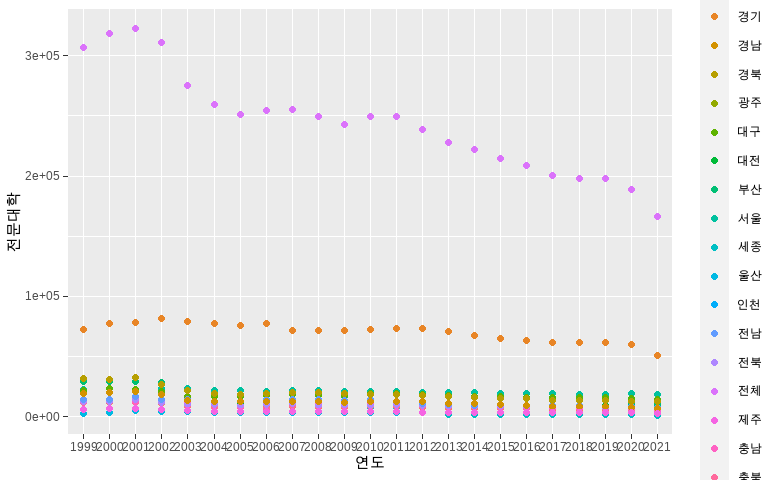
\includegraphics[width=1\linewidth]{chap4_files/figure-latex/unnamed-chunk-4-1}
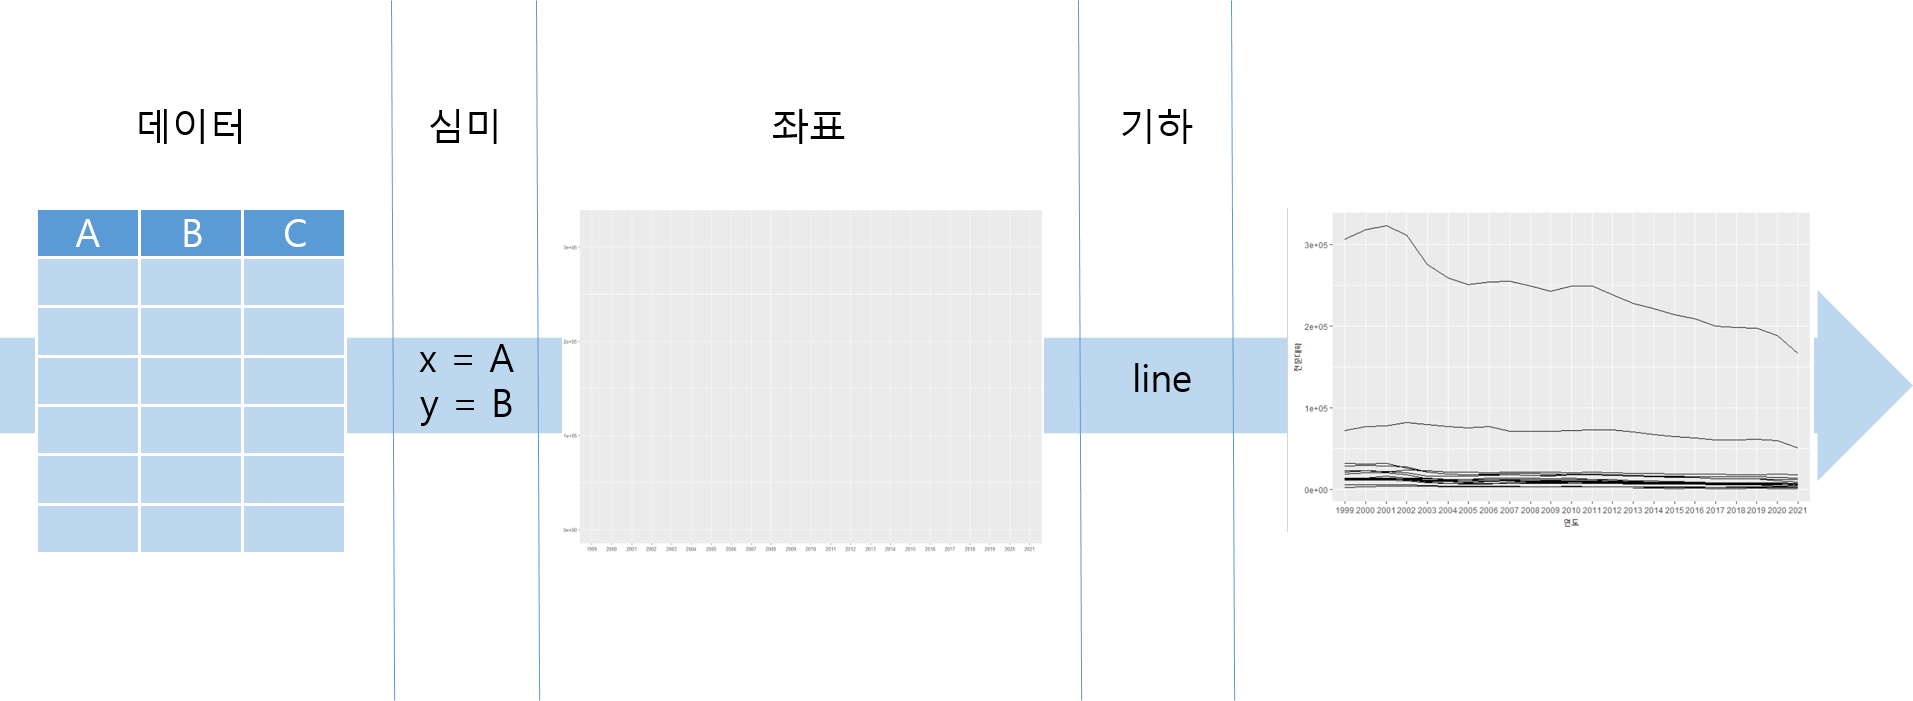
\includegraphics{그림1.emf}

\end{document}
